% main5.tex -- H-main.  Section 5: getting started -- the touch-down theorem (proved in Appendix B).
%======================================================================
\section{Getting started: the front at touch-down}\label{sec:touchdown}
%======================================================================

The end theorem needs a front that is flat on all scales between $\varepsilon$ and $R$, whose chords are not too short,
and which starts exactly at Harry. Design~T produces such a front, and the reason we can \emph{prove} it is that both of
its runs are straight. On a straight run the motion of a single candidate is completely explicit, so the front at
touch-down can be described almost in closed form, and its tangent and curvature can be followed exactly along each
run. This is what makes the starting data of the bootstrap provable.

\textbf{Two conserved quantities.} Put Harry at the origin, moving with unit velocity in the direction $1\in\C$, and
write a candidate as $r=\rho e^{i\beta}$ relative to him. Then $r'=v\hat r-1$, that is,
\[
\rho'=v-\cos\beta,\qquad \rho\beta'=\sin\beta .
\]
Two combinations are remarkably simple: $h:=\rho(\cos\beta+v)$ decreases at the constant rate $1-v^2$, and
\[
\mathcal C:=\rho\,\frg(\beta),\qquad \frg(\beta):=\frac{\sin\beta}{\tan^v(\beta/2)},
\]
is constant (check: $(\log\rho)'=(v-\cos\beta)/\rho$ and $(\log\frg(\beta))'=\frac{\cos\beta-v}{\sin\beta}\,\beta'=
(\cos\beta-v)/\rho$). So every candidate moves along an explicit curve, and its position at any time on the run is found
by solving $h(t)=h(t_1)-(1-v^2)(t-t_1)$ for $\beta$. Differentiating these formulas in the direction label $\alpha$
gives the tangent, the stretching and the curvature of the front, again exactly. Appendix~B carries this out for the two
runs of Design~T, by perturbing from $v=0$, where the front is the unit circle.

\textbf{What happens near the touch-down point.} Because run~2 is tangent to the front, the candidates on either side of
$\alpha_0$ are approached at a grazing angle. The bearing of candidate $\alpha_0\pm\xi$ from Harry has a double zero at
$\xi=0$, so these candidates come within distance about $\xi^2$ of Harry's line. Those on the forward side are still
ahead of Harry at touch-down; they form the forward arc, which starts exactly at Harry and leaves along his heading
$\hat n$. Those on the backward side were passed: the ones with $\xi^2\lesssim\varepsilon$ came within $\varepsilon$ of
Harry and are seen; the others form the tail arc, whose end lies at distance $z_0\asymp\varepsilon^{1/(2-2v)}$
(roughly $\varepsilon^{1/2}$) behind Harry, also pointing along $\hat n$ (Figure~\ref{fig:touchdown}). The rest of the
front is far from Harry and smooth; only the small hole around direction $0$, cut by run~1, needs a separate argument.

\begin{figure}[!htbp]
\centering
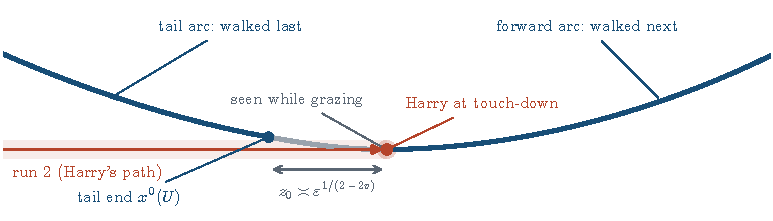
\includegraphics[width=0.92\linewidth]{figs/fig_touchdown.pdf}
\caption{The front at touch-down, seen from Harry, with his heading pointing right ($v=0.1$, $\varepsilon=0.01$,
simulated). Harry has run along a tangent to the front; the shaded band is the strip of width $2\varepsilon$ he has
searched. The forward arc starts at Harry; a sliver of length $\asymp\varepsilon^{1/(2-2v)}$ (roughly
$\varepsilon^{1/2}$) behind him has been seen while grazing; the tail end $x^0(U)$, the last point of the walk, lies at
distance $z_0\asymp\varepsilon^{1/(2-2v)}$ behind Harry and points along his path.}
\label{fig:touchdown}
\end{figure}

We now state precisely what Appendix~B proves. The front at touch-down is assembled from three kinds of labels:
virtual candidates in a window of width $\xi_1\varepsilon$ just ahead of $\alpha_0$ (they have been inside the vision disc,
and only their virtual versions are used), true candidates everywhere else, and one limit point $Z_s$ that fills the hole
left by run~1 at direction $0$. Two quantities from Appendix~B appear in the statement. The constant $\xi_1$ is chosen
so that every candidate $\alpha_0+\xi$ with $\xi\ge\xi_1\varepsilon$ stays at distance at least $2\varepsilon$ from Harry
up to $t_\td$ (Lemma~\ref{lem:B-forward}(d)); so only the window $[\alpha_0,\alpha_0+\xi_1\varepsilon)$ can contain
candidates that came within $\varepsilon$ of Harry on the forward side. The label $\be:=\alpha_0-\xie$ is the boundary
direction of the sliver seen while grazing: it is the tail direction whose minimal distance from Harry during run~2 is
exactly $\varepsilon$, i.e.\ $\mathcal C(\be)=\varepsilon\gmax$ for its run-2 integral, where $\gmax:=\max\frg$
(so $\mathcal C/\gmax$ is the minimum of $\rho=\mathcal C/\frg(\beta)$ on a run), and $\xie\asymp\varepsilon^{1/(2-2v)}$
(Lemma~\ref{lem:B-tail}(a)).

\begin{theorem}[Front at touch-down]\label{thm:touchdown}
There is an absolute $\lambda_*>0$ such that for every $\lambda_0\in(0,\lambda_*]$ there exist
$c_{\mathrm{sep}}=c_{\mathrm{sep}}(\lambda_0)>0$ and $\varepsilon_{\mathrm T}=\varepsilon_{\mathrm T}(\lambda_0)>0$
\textup(independent of $v$ and $\varepsilon$\textup), and absolute constants $v_{\mathrm T},\xi_1,G_T,\kappa_c,
C_{\mathrm{td}}>0$ \textup(independent of $\lambda_0$\textup), such that for all $v\in(0,v_{\mathrm T}]$ and
$\varepsilon\in(0,\varepsilon_{\mathrm T}(\lambda_0)]$ the following holds under Design~T, with $d=1$. First,
$t_\td=2+\sqrt3+O(v+\varepsilon)\le4$. Define $\Upsilon(\alpha)$ for
$\alpha\in[\alpha_0,2\pi+\be]$ \textup(directions taken mod $2\pi$\textup) as $x_\alpha(t_\td)$ on
$[\alpha_0,\alpha_0+\xi_1\varepsilon]$, as $S_\alpha(t_\td)$ on $[\alpha_0+\xi_1\varepsilon,2\pi+\be]\setminus\{2\pi\}$,
and as $Z_s:=\lim_{\alpha\to0^\pm}S_\alpha(t_\td)$ at $2\pi$. Its arclength reparametrisation $x^0:[0,U]\to\R^2$,
$x^0(u)=\Upsilon(\Theta(u))$, is $C^1$ with $|\partial_ux^0|\equiv1$, $|U-2\pi|\le C_{\mathrm{td}}(v+\varepsilon^{1/2})$ and $1\le U\le8$
\textup(the seen directions $(\be,\alpha_0)$, an interval of length $\xie$, are cut off\textup). Labels are arclength at
$t_\td$, quantities below are evaluated at $t_\td$, and:
\begin{itemize}
\setlength{\itemsep}{1pt}\setlength{\parskip}{0pt}
\item[\textup{(T0)}] $x^0(0)=P(t_\td)$; every $u\notin\mathcal G$ is true \textup(with direction $\Theta(u)$\textup), where
$\mathcal G$ is the set of labels with $\Theta(u)=2\pi$ or $\Theta(u)\in[\alpha_0,\alpha_0+\xi_1\varepsilon)$; for
$u\in\mathcal G$ the direction $\Theta(u)$ is seen by $t_\td$ or $u$ is true; and every $\theta\in[0,2\pi)$ is seen by
$t_\td$ or carried by a true label;
\item[\textup{(T1)}] $N(a,b)\le C_{\mathrm{td}}\lambda^{3/2-\mu_T}$ for all pairs with $\varepsilon/2\le\lambda\le\lambda_0$;
\item[\textup{(T2)}] $c(a,b)\ge\min\bigl(c_{\mathrm{sep}}(\lambda_0),\,\kappa_c(a+U-b)\bigr)$ for all pairs with $\lambda>\lambda_0$;
\item[\textup{(T3)}] $|T(u)-\hat n|\le C_{\mathrm{td}}u^{1-\mu}$ for $u\le G_T$;
\item[\textup{(T4)}] $|T(u)-\hat n|\le C_{\mathrm{td}}(U-u+z_0)^{1-\mu_T}$ for $U-u\le G_T$;
\item[\textup{(T5)}] $P(t_\td)-x^0(U)=z_0\hat n+y_0\hat n^\perp$ with $z_0\asymp\varepsilon^{1/(2-2v)}$
\textup(that is, $c\,\varepsilon^{1/(2-2v)}\le z_0\le C_{\mathrm{td}}\varepsilon^{1/(2-2v)}$ for an absolute $c>0$\textup)
and $|y_0|\le C_{\mathrm{td}}(z_0+\varepsilon)^{2-\mu_T}$.
\end{itemize}
\end{theorem}

In words: (T0) the front starts at Harry and accounts for every direction; (T1) it is flat on small scales, with a
bendiness exponent $\frac32-\mu_T$ just below the value $\frac32$ of a smooth curve; (T2) two points far apart along the
front are far apart in the plane, unless they are the two ends, which are close to each other; (T3)--(T4) both ends
leave along Harry's heading $\hat n$; (T5) the tail end is behind Harry, at a distance much larger than $\varepsilon$
but tending to zero with $\varepsilon$. Appendix~C (Lemma~\ref{lem:startchord}) turns (T1)--(T2) into the start
conditions (S1)--(S2) of Setting~(H) for the body pairs. The pairs near the tail end are the excused tail pairs of
Setting~(H); they are dealt with in the next section.

